% main.tex
% 湖州学院开题答辩 Beamer 模板
% 基于 metropolis 主题的现代极简设计

\documentclass[aspectratio=169, 10pt]{beamer}

% Engine guard (Overleaf should use LuaLaTeX)
\RequirePackage{iftex}
\ifLuaTeX\else\ifXeTeX\else
  \PackageError{Beamer}{This project requires LuaLaTeX (or XeLaTeX)}{In Overleaf: Menu -> Settings -> Compiler -> LuaLaTeX.}
  \endinput
\fi\fi

\usepackage[UTF8,fontset=fandol]{ctex}

% Tabular extensions (must be loaded before colortbl)
\usepackage{array}

% Compatibility shim: newer `array` uses \insert@column for p/m/b columns,
% while `colortbl` may still refer to \insert@pcolumn.
\makeatletter
\providecommand\insert@pcolumn{\insert@column}
\makeatother

% Table row colors (\rowcolor) support
\usepackage{colortbl}

%% ============ 颜色定义 ============
% AI‑Native Minimal (Neutral base + single accent color)
% 别用 #FFFFFF,太死板。用 #FBFBFD,这是 Apple 官网的背景白。
\definecolor{bg}{HTML}{FBFBFD}
% 卡片背景不要太灰,要极其微妙,像纸张微微隆起。
\definecolor{bgsoft}{HTML}{F5F5F7}
% 别用纯黑。用 #1D1D1F,这是 Apple 的标准字色,深邃但不死黑。
\definecolor{ink}{HTML}{1D1D1F}
% 次要文字用冷灰,增加科技感。
\definecolor{slate}{HTML}{424245}
% 辅助文字(页脚/引用)用中性灰。
\definecolor{muted}{HTML}{86868B}
% 线条要几乎看不见,但又确实存在。
\definecolor{line}{HTML}{D2D2D7}
% Single accent: AI Indigo (Tailwind indigo-500-ish). Keep everything else neutral.
\definecolor{accent}{HTML}{6366F1}
\colorlet{accentSoft}{accent!10}
\colorlet{accentLine}{accent!35}

%% ============ 主题与配置 ============
\usetheme{metropolis}
% Remove section title pages and progress bar; keep fraction numbering.
\metroset{progressbar=none, numbering=fraction, sectionpage=none}

% Core palette
\setbeamercolor{normal text}{fg=ink, bg=bg}
\setbeamercolor{alerted text}{fg=accent}
\setbeamercolor{title}{fg=ink}
\setbeamercolor{subtitle}{fg=slate}
\setbeamercolor{author}{fg=ink}
\setbeamercolor{institute}{fg=muted}
\setbeamercolor{date}{fg=muted}

% Metropolis internals
\setbeamercolor{progress bar}{fg=accent, bg=line}
\setbeamercolor{title separator}{fg=accent}
\setbeamercolor{frametitle}{fg=ink, bg=bg}
\setbeamercolor{palette primary}{fg=ink, bg=bg}
\setbeamercolor{palette secondary}{fg=ink, bg=bg}
\setbeamercolor{palette tertiary}{fg=ink, bg=bg}
\setbeamercolor{palette quaternary}{fg=ink, bg=bg}
\setbeamercolor{structure}{fg=accent}

% Typography scale (Apple-like: big titles + whitespace)
\setbeamerfont{title}{size=\Huge, series=\bfseries}
% 别用 \mdseries,副标题也要有分量,但用颜色区分。
\setbeamerfont{subtitle}{size=\Large, series=\bfseries}
\setbeamerfont{frametitle}{size=\LARGE, series=\bfseries}

%% ============ 字体配置(LuaLaTeX / XeLaTeX) ============
\usepackage{fontspec}

% 英文无衬线字体(带 fallback)
\IfFontExistsTF{TeX Gyre Heros}{
  \setsansfont{TeX Gyre Heros}
  \setmainfont{TeX Gyre Heros}
}{
  \setsansfont{Latin Modern Sans}
  \setmainfont{Latin Modern Sans}
}

% CJK fonts are handled by `ctex` (fontset=fandol) for maximum portability.
% Set a CJK monofont to avoid warnings when using \ttfamily.
\ifdefined\setCJKmainfont
  % Prefer a clean CJK sans look when available (portable within Fandol set).
  \IfFontExistsTF{FandolHei}{
    \setCJKmainfont{FandolHei}
    \setCJKsansfont{FandolHei}
  }{}
\fi
\ifdefined\setCJKmonofont
  \IfFontExistsTF{FandolFang}{
    \setCJKmonofont{FandolFang}
  }{}
\fi

% 字体大小设置
\usepackage{setspace}
% 1.15 太挤了,这是对观众视力的侮辱。改成 1.3,让文字呼吸。
\setstretch{1.22}

%% ============ 页面设置 ============
% 去掉 navigation symbols
\setbeamertemplate{navigation symbols}{}
\setbeamertemplate{headline}{}

% Minimal Apple-like footer (page number only)
\setbeamertemplate{footline}{
  \begin{beamercolorbox}[wd=\paperwidth, ht=0.5cm, dp=0.2cm, leftskip=1.1cm, rightskip=1.1cm]{footline}
    \hfill{\color{muted}\footnotesize\insertframenumber/\inserttotalframenumber}
  \end{beamercolorbox}
}

% Blocks
\setbeamercolor{block title}{fg=ink, bg=bgsoft}
\setbeamercolor{block body}{fg=slate, bg=bgsoft}
\setbeamercolor{block title alerted}{fg=ink, bg=bgsoft}
\setbeamercolor{block body alerted}{fg=slate, bg=bgsoft}
\setbeamertemplate{blocks}[rounded][shadow=false]

% Lists
\setbeamertemplate{itemize item}{\color{accent}\small$\bullet$}
\setbeamertemplate{itemize subitem}{\color{muted}\tiny$\bullet$}
\setlength{\leftmargini}{1.2em}
\setlength{\leftmarginii}{1.1em}

%% ============ 参考文献配置 ============
\usepackage[backend=biber, style=numeric, sorting=none]{biblatex}
\addbibresource{refs.bib}

%% ============ 代码块配置 ============
\usepackage{listings}
\lstset{
    basicstyle=\ttfamily\small,
    keywordstyle=\color{accent}\bfseries,
    commentstyle=\color{muted},
    stringstyle=\color{ink},
    numbers=left,
    numberstyle=\tiny\color{muted},
    frame=single,
    framerule=0.5pt,
    rulecolor=\color{line},
    backgroundcolor=\color{bgsoft},
    tabsize=4,
    showspaces=false,
    showstringspaces=false,
    breaklines=true,
    linewidth=0.9\textwidth,
    xleftmargin=0.05\textwidth,
    xrightmargin=0.05\textwidth
}

%% ============ TikZ 包 ============
\usepackage{tikz}
\usetikzlibrary{positioning, shapes, arrows, calc}

%% ============ AI‑Native components (pills / cards / bento) ============
% Keep the deck consistent: every page should reuse the same small set of components.
\usepackage{xparse}
\NewDocumentCommand{\pill}{m}{%
  \tikz[baseline=(P.base)]\node[
    draw=line,
    fill=bgsoft,
    rounded corners=2.6mm,
    line width=0.45pt,
    inner xsep=6.5pt,
    inner ysep=3.2pt,
    font=\sffamily\scriptsize\bfseries,
    text=slate
  ] (P) {#1};%
}
\NewDocumentCommand{\pillaccent}{m}{%
  \tikz[baseline=(P.base)]\node[
    draw=accentLine,
    fill=accentSoft,
    rounded corners=2.6mm,
    line width=0.55pt,
    inner xsep=6.5pt,
    inner ysep=3.2pt,
    font=\sffamily\scriptsize\bfseries,
    text=accent
  ] (P) {#1};%
}
\NewDocumentCommand{\framepills}{m}{%
  \vspace{-0.55em}%
  \noindent #1\par
  \vspace{0.55em}%
}
% Verbatim-safe card wrapper (supports listings / lstlisting inside).
% Implementation note: avoid grabbing the environment body as a macro argument.
% Important: `block` uses `\textwidth` internally; wrap it in a minipage so
% `\textwidth` becomes the current column width inside `columns`.
\newenvironment{aicard}[1][]{%
  \begin{minipage}{\linewidth}
    \begin{block}{#1}
}{%
    \end{block}
  \end{minipage}
}

%% ============ 表格样式 ============
\usepackage{booktabs}
\newcolumntype{L}{>{\raggedright\arraybackslash}p{0.45\textwidth}}
\newcolumntype{C}{>{\centering\arraybackslash}p{0.25\textwidth}}
\newcolumntype{R}{>{\raggedleft\arraybackslash}p{0.25\textwidth}}

%% ============ 数学公式 ============
\usepackage{amsmath, amsthm, amssymb}

%% ============ 标题信息(请修改以下内容) ============
% Personal meta (fill with your real info)
\newcommand{\studentname}{沈佳豪}
% Light, consistent form line placeholder (Apple-like).
% Uses a subtle gray rule so empty fields don't look visually "heavy".
\newcommand{\formline}[1]{\textcolor{line}{\rule[-0.2ex]{#1}{0.6pt}}}
\newcommand{\studentid}{\formline{3.2cm}}
\newcommand{\studentmajor}{\formline{3.2cm}}
\newcommand{\advisor}{\formline{3.2cm}}

% Cover display title (manual line break to avoid awkward CJK wrapping).
\newcommand{\covertitle}{\mbox{基于 LangGraph 的法律智能体}\\系统设计与实现}

% Keep `\title{...}` single-line for PDF metadata / navigation.
\title{基于 LangGraph 的法律智能体系统设计与实现}
\subtitle{自建 LangGraph + RAG · 开题答辩}
\author{\studentname}
\institute{湖州学院 \quad 计算机科学与技术学院}
\date{\today}

%% ============ 校徽路径接口 ============
% 如果 assets/hzu-logo.png 不存在,将使用 TikZ 占位框
% 请将真实校徽图片放在 assets/hzu-logo.png

\begin{document}

% 封面
% sections/00-cover.tex
% 封面页

\begin{frame}[plain]
    \begin{tikzpicture}[remember picture, overlay]
        % Background (Apple Light)
        \fill[bg] (current page.south west) rectangle (current page.north east);

        % Top meta
        \node[anchor=north west] at ($(current page.north west) + (1.1cm, -0.9cm)$) {
            % \sffamily 才是优雅的。两个单词之间用 · 分隔,而不是程序员的 //
            {\sffamily\fontsize{8}{12}\selectfont\color{muted}\textbf{EQUIVOCAL LEGAL} \quad $\cdot$ \quad \textbf{PROPOSAL DEFENSE}}
        };

        % Minimal HZU badge (fallback if no logo asset)
        \node[anchor=north east] at ($(current page.north east) + (-1.1cm, -0.85cm)$) {
            \tikz[baseline] \node[
                draw=line,
                fill=bgsoft,
                rounded corners=2mm,
                minimum width=1.35cm,
                minimum height=0.62cm,
                font=\fontsize{9}{11}\selectfont\bfseries,
                text=ink
            ] {HZU};
        };

        % Title & subtitle (split from pills so the underline never falls into the meta card area)
        \node[anchor=west, text width=0.84\textwidth, align=left] (title_node) at ($(current page.west) + (1.1cm, 1.55cm)$) {
            {\fontsize{25}{31}\selectfont\bfseries\color{ink}\covertitle}\par
            \vspace{0.30cm}
            {\fontsize{14}{18}\selectfont\color{slate}\insertsubtitle}\par
        };

        % Accent underline (belongs to title area)
        \draw[accent, line width=1.6pt] ($(title_node.south west) + (0, -0.05cm)$) -- ++(2.8cm, 0);

        % Pills (kept visually close to subtitle, but independent from underline)
        \node[anchor=north west, text width=0.84\textwidth, align=left] (pills_node) at ($(title_node.south west) + (0, -0.18cm)$) {
            {\pillaccent{LangGraph}\hspace{0.15cm}\pill{RAG}\hspace{0.15cm}\pill{Legal AI}\hspace{0.15cm}\pill{Traceable}}
        };

        % Bottom-left meta card
        \node[anchor=south west] at ($(current page.south west) + (1.1cm, 0.9cm)$) {
            \begin{tikzpicture}
                \node[draw=line, fill=bgsoft, rounded corners=3.2mm, line width=0.55pt, inner sep=10pt] (meta) {
                    \begin{minipage}{0.68\textwidth}
                        {\fontsize{11}{14}\selectfont\color{ink}\textbf{姓名:}\studentname}\par
                        \vspace{0.12cm}
                        {\fontsize{11}{14}\selectfont\color{ink}\textbf{学号:}\studentid}\par
                        \vspace{0.12cm}
                        {\fontsize{11}{14}\selectfont\color{ink}\textbf{学院/专业:}\studentmajor}\par
                        \vspace{0.12cm}
                        {\fontsize{11}{14}\selectfont\color{ink}\textbf{指导教师:}\advisor}\par
                        \vspace{0.28cm}
                        {\fontsize{10}{13}\selectfont\color{muted}\insertinstitute \quad · \quad \insertdate}
                    \end{minipage}
                };
            \end{tikzpicture}
        };
    \end{tikzpicture}
\end{frame}


% 目录
% sections/01-toc.tex
% 目录页

\section{目录}

\begin{frame}{目录}
    \framepills{\pillaccent{Agenda}\hspace{0.15cm}\pill{AI‑Native Minimal}\hspace{0.15cm}\pill{Traceable MVP}}

    \begin{columns}[T, onlytextwidth]
        \begin{column}{0.62\textwidth}
            \begin{aicard}[Narrative]
                \begin{enumerate}\setlength{\itemsep}{0.28cm}
                    \item 背景与问题定义:为什么需要法律智能体
                    \item 目标与边界:面向可验收的 MVP
                    \item 系统方案:LangGraph + RAG 的工程化落地
                    \item 实验设计:验收指标与风险对策
                    \item 计划与预期成果:里程碑与交付物
                \end{enumerate}
            \end{aicard}
        \end{column}
        \begin{column}{0.38\textwidth}
            \begin{aicard}[Audience takeaway]
                \begin{itemize}\setlength{\itemsep}{0.28cm}
                    \item 这不是“聊天机器人”,而是\textbf{工程化流程}
                    \item 关键输出可\textbf{追溯/回放/审计}
                    \item 上游失败时可\textbf{降级}而非沉默
                \end{itemize}
            \end{aicard}
        \end{column}
    \end{columns}
\end{frame}


% 研究背景
% sections/02-background.tex
% 研究背景

\section{背景与问题}

\begin{frame}[c]{背景与意义:为什么需要法律智能体}
    \framepills{\pillaccent{Problem}\hspace{0.15cm}\pill{Cost}\hspace{0.15cm}\pill{Risk}\hspace{0.15cm}\pill{Fragmented info}}

    \begin{columns}[T, onlytextwidth]
        \begin{column}{0.58\textwidth}
            \begin{aicard}[User pain]
                \begin{itemize}\setlength{\itemsep}{0.32cm}
                    \item \textbf{成本高、门槛高}:依赖专业人力;用户常常“问不到点子上”
                    \item \textbf{风险点隐蔽}:条款风险埋在细节里,误解可能带来高代价
                    \item \textbf{信息碎片化}:法条/案例/流程分散,检索与比对成本高
                \end{itemize}
            \end{aicard}
        \end{column}
        \begin{column}{0.42\textwidth}
            \begin{aicard}[Why now]
                \textbf{大模型}带来自然语言交互能力,\textbf{RAG}把回答与依据绑定,让关键结论\textbf{可追溯、可复核}\cite{lewis2020rag}。\par
                \vspace{0.35em}
                {\footnotesize\color{muted}目标不是“更会聊天”,而是“更可验收”。}
            \end{aicard}
        \end{column}
    \end{columns}
\end{frame}

\begin{frame}[c]{问题定义:把“咨询”工程化到可验收}
    \framepills{\pillaccent{Definition}\hspace{0.15cm}\pill{MVP}\hspace{0.15cm}\pill{Traceable}\hspace{0.15cm}\pill{Safe boundary}}

    \begin{columns}[T, onlytextwidth]
        \begin{column}{0.52\textwidth}
            \begin{aicard}[One‑sentence mission]
                让用户在 3 分钟内得到\textbf{可执行的下一步}(需要补充哪些事实 / 风险点在哪里 / 建议怎么做),并保证\textbf{可追溯、可回放、可验收}。
            \end{aicard}
        \end{column}
        \begin{column}{0.48\textwidth}
            \begin{aicard}[Boundaries \& principles]
                \begin{itemize}\setlength{\itemsep}{0.26cm}
                    \item \textbf{不替代律师}:输出建议与依据,提示适用范围与不确定性
                    \item \textbf{可追溯}:关键输出绑定 traceId / 模型信息 / 引用来源
                    \item \textbf{可降级}:上游不可用时返回结构化替代步骤(非“报错/沉默”)
                    \item \textbf{隐私最小化}:最小化存储、可选脱敏,避免泄露敏感信息
                \end{itemize}
            \end{aicard}
        \end{column}
    \end{columns}
\end{frame}


% 研究方法
% sections/03-methodology.tex
% 研究方法

\section{系统方案}

\begin{frame}[t]{系统方案:LangGraph + RAG 的工程化落地}
    \framepills{\pillaccent{Architecture}\hspace{0.15cm}\pill{Next.js}\hspace{0.15cm}\pill{Java Gateway}\hspace{0.15cm}\pill{LangGraph}\hspace{0.15cm}\pill{RAG}}
    \vspace{-0.30cm}

    \begin{columns}[T, onlytextwidth]
        \begin{column}{0.54\textwidth}
            \begin{aicard}[Components]
                \begin{itemize}\setlength{\itemsep}{0.16cm}
                    \item \textbf{前端(Next.js)}:对话 UI、服务类型入口、SSE 流式渲染
                    \item \textbf{后端(Java)}:JWT 鉴权、会话管理、审计留痕、限流/风控
                    \item \textbf{智能体(FastAPI + LangGraph)}:多步推理 + 工具调用,必要时检索引用\cite{langgraph2024}
                    \item \textbf{数据层}:向量检索(Cloudflare Vectorize)+ 文件存储(R2)+ 结构化日志(DB)
                \end{itemize}
                {\footnotesize\color{muted}目标:把“咨询”变成可追溯的工程流程。}
            \end{aicard}
        \end{column}
        \begin{column}{0.46\textwidth}
            \begin{aicard}[Flow]
                \centering
                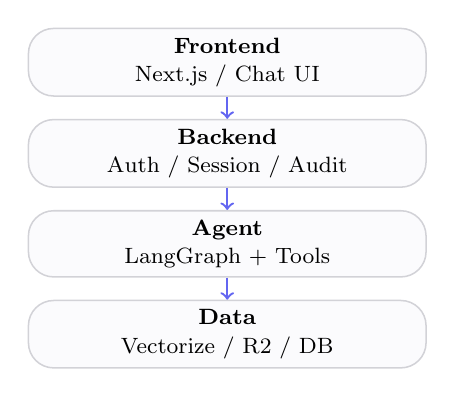
\begin{tikzpicture}[node distance=0.58cm, every node/.style={font=\fontsize{8.2}{10.2}\selectfont, align=center}]
                    \node[rounded corners=3.2mm, draw=line, fill=bg, line width=0.55pt, minimum width=5.05cm, minimum height=0.80cm] (fe) {\textbf{Frontend}\\ Next.js / Chat UI};
                    \node[rounded corners=3.2mm, draw=line, fill=bg, line width=0.55pt, minimum width=5.05cm, minimum height=0.80cm, below=0.28cm of fe] (be) {\textbf{Backend}\\ Auth / Session / Audit};
                    \node[rounded corners=3.2mm, draw=line, fill=bg, line width=0.55pt, minimum width=5.05cm, minimum height=0.80cm, below=0.28cm of be] (ai) {\textbf{Agent}\\ LangGraph + Tools};
                    \node[rounded corners=3.2mm, draw=line, fill=bg, line width=0.55pt, minimum width=5.05cm, minimum height=0.80cm, below=0.28cm of ai] (data) {\textbf{Data}\\ Vectorize / R2 / DB};

                    \draw[->, line width=0.85pt, color=accent] (fe) -- (be);
                    \draw[->, line width=0.85pt, color=accent] (be) -- (ai);
                    \draw[->, line width=0.85pt, color=accent] (ai) -- (data);
                \end{tikzpicture}
            \end{aicard}
        \end{column}
    \end{columns}
\end{frame}

\begin{frame}[t, fragile]{关键流程:工具调用 + 引用 + 追溯(traceId)}
    \framepills{\pillaccent{Trace}\hspace{0.15cm}\pill{Tools}\hspace{0.15cm}\pill{Citations}\hspace{0.15cm}\pill{Replayable}}

    \begin{columns}[T, onlytextwidth]
        \begin{column}{0.54\textwidth}
            \begin{aicard}[Request pipeline]
                \begin{itemize}\setlength{\itemsep}{0.24cm}
                    \item \textbf{Input}:问题/合同片段(可选脱敏)+ 用户身份
                    \item \textbf{Guard}:鉴权、限流、风险提示模板
                    \item \textbf{Agent}:决策(检索/生成/追问)
                    \item \textbf{Tools}:RAG / OCR / 文书生成
                    \item \textbf{Output}:建议 + 免责声明 +(可选)引用 + traceId
                \end{itemize}
            \end{aicard}
        \end{column}
        \begin{column}{0.46\textwidth}
            \begin{aicard}[LangGraph (pseudo)]
                \lstset{language=Python, basicstyle=\ttfamily\scriptsize, numbers=none, frame=none, backgroundcolor=\color{bg}, linewidth=\linewidth, xleftmargin=0pt, xrightmargin=0pt}
                \begin{lstlisting}
graph = StateGraph(State)
graph.add_node("decide", decide)
graph.add_node("rag", legal_rag_search)
graph.add_edge("decide", "rag")
graph.add_edge("rag", "decide")
graph.compile()
                \end{lstlisting}
                {\footnotesize\color{muted}要点:把多步推理固定为图结构,便于测试与回放。}
            \end{aicard}
        \end{column}
    \end{columns}
\end{frame}


% 实验与结果
% sections/04-experiments.tex
% 实验与结果

\section{实验与验收}

\begin{frame}[c]{核心能力与服务类型(MVP)}
    \framepills{\pillaccent{MVP}\hspace{0.15cm}\pill{Contract review}\hspace{0.15cm}\pill{Drafting}\hspace{0.15cm}\pill{Consulting}}

    \begin{aicard}[Service types]
        {\small
        \renewcommand{\arraystretch}{1.01}
        \begin{tabular}{p{0.28\textwidth} p{0.66\textwidth}}
            \toprule
            \textbf{服务类型} & \textbf{典型输出} \\
            \midrule
            合同审查 & 风险点 + 修改建议 +(可选)引用依据 \\
            合同生成/保密协议/借条/租赁合同 & 结构化信息收集 + 文书草案 + 风险提示 \\
            \rowcolor{accentSoft}
            法律咨询 & 追问补全事实 + 可执行下一步 + 边界声明 \\
            \bottomrule
        \end{tabular}
        }
    \end{aicard}

    \vspace{0.05cm}
    \begin{aicard}[Why tools matter]
        {\footnotesize 工具让智能体能\textbf{检索引用、生成文书、做 OCR},并把多步推理固定成可验证的流程(而不是一次性生成)\cite{yao2022react}。}
    \end{aicard}
\end{frame}

\begin{frame}[c]{验收指标:可用、可追溯、可降级}
    \framepills{\pillaccent{Acceptance}\hspace{0.15cm}\pill{Available}\hspace{0.15cm}\pill{Traceable}\hspace{0.15cm}\pill{Degradable}}

    \begin{columns}[T, onlytextwidth]
        \begin{column}{0.5\textwidth}
            \begin{aicard}[Availability]
                \textbf{关键接口}可用性 $\ge$ 99\%;失败可定位(错误码 + traceId)。
            \end{aicard}
            \vspace{0.32cm}
            \begin{aicard}[Traceability]
                会话/消息/关键输出可检索(provider / model / latency / tokens)。
            \end{aicard}
        \end{column}
        \begin{column}{0.5\textwidth}
            \begin{aicard}[Latency]
                流式输出首 token 体验优先;常见请求 < 2s(按环境调参)。
            \end{aicard}
            \vspace{0.32cm}
            \begin{aicard}[Fallback \& boundary]
                检索失败/模型不可用时返回“下一步要补充的信息清单”,并提示不确定性与适用范围。
            \end{aicard}
        \end{column}
    \end{columns}
\end{frame}


% 结论与展望
% sections/05-conclusion.tex
% 结论与展望

\section{计划与成果}

\begin{frame}[c]{阶段性成果(当前进展)}
    \framepills{\pillaccent{Progress}\hspace{0.15cm}\pill{MVP ready}\hspace{0.15cm}\pill{Engineering-first}}

    \begin{columns}[T, onlytextwidth]
        \begin{column}{0.5\textwidth}
            \begin{aicard}[Product]
                多服务类型入口(合同审查 / 文书生成 / 法律咨询),围绕“\textbf{可执行下一步}”。
            \end{aicard}
            \vspace{0.28cm}
            \begin{aicard}[System]
                前端(Next.js)+ 后端(Java)+ 智能体(FastAPI + LangGraph)链路成型。
            \end{aicard}
        \end{column}
        \begin{column}{0.5\textwidth}
            \begin{aicard}[RAG infra]
                向量库(Cloudflare Vectorize)+ 文件存储(R2),支持引用与材料上传。
            \end{aicard}
            \vspace{0.28cm}
            \begin{aicard}[Acceptance baseline]
                追溯字段、审计日志、失败降级策略,支持\textbf{可验收与可复盘}。
            \end{aicard}
        \end{column}
    \end{columns}
\end{frame}

\begin{frame}[c]{计划与预期成果(W1–W8)}
    \framepills{\pillaccent{Roadmap}\hspace{0.15cm}\pill{W1–W8}\hspace{0.15cm}\pill{Deliverables}}

    \begin{columns}[T, onlytextwidth]
        \begin{column}{0.56\textwidth}
            \begin{aicard}[Milestones]
                \begin{itemize}\setlength{\itemsep}{0.14cm}
                    \item W1–W2:用例与数据结构定稿;会话/审计表结构;关键页面原型
                    \item W3–W4:Java 网关与鉴权完善;SSE 流式链路;端到端联调
                    \item W5–W6:智能体策略(追问/检索/生成);降级与风控;引用输出规范
                    \item W7:测试与验收脚本(合同审查/劳动争议/文书生成)
                    \item W8:论文与答辩材料;演示脚本与彩排
                \end{itemize}
            \end{aicard}
        \end{column}
        \begin{column}{0.44\textwidth}
            \begin{aicard}[Deliverables]
                \begin{itemize}\setlength{\itemsep}{0.14cm}
                    \item 可演示 MVP:登录 + 咨询 + 留痕 + 可追溯引用
                    \item 关键场景 Demo:合同审查 / 文书生成 / 法律咨询
                    \item 可验收口径:指标 + 日志 + traceId 回放 + 风险对策
                \end{itemize}
            \end{aicard}
        \end{column}
    \end{columns}
\end{frame}


% 致谢
% sections/06-acknowledgements.tex
% 致谢

\section{致谢}

\begin{frame}[plain]
    \begin{tikzpicture}[remember picture, overlay]
        \fill[bg] (current page.south west) rectangle (current page.north east);

        \node[anchor=center] at ($(current page.center) + (0, 0.4cm)$) {
            {\fontsize{54}{60}\selectfont\bfseries\color{ink}Q \& A}
        };
        \node[anchor=center] at ($(current page.center) + (0, -0.55cm)$) {
            {\fontsize{18}{24}\selectfont\color{slate}谢谢。欢迎提问与质疑我的边界与验收口径。}
        };
        \node[anchor=center] at ($(current page.center) + (0, -1.25cm)$) {
            {\pillaccent{Questions}\hspace{0.15cm}\pill{Boundary}\hspace{0.15cm}\pill{Acceptance}}
        };

        \draw[accent, line width=1.6pt] ($(current page.south) + (-2.2cm, 1.45cm)$) -- ++(4.4cm, 0);
    \end{tikzpicture}
\end{frame}


% 参考文献
% sections/07-references.tex
% 参考文献

\appendix
\section{参考文献}

\begin{frame}[allowframebreaks]{参考文献}
    \framepills{\pillaccent{References}\hspace{0.15cm}\pill{LangGraph}\hspace{0.15cm}\pill{RAG}\hspace{0.15cm}\pill{Legal NLP}}
    \begin{spacing}{1.2}
        \printbibliography[heading=none]
    \end{spacing}
\end{frame}


\end{document}
